%!TEX root = spire-project.tex
\subsection{Using Spitzer Image}

Assuming a possible twofold increase in angular resolution when using HiRes, the ideal source of a truth image would be to have a telescope observing at the same wavelengths as Herschel, but with a mirror of twice the diameter. Obviously such a telescope does not exist so another source of truth images is needed, and without a physical source then we need a simulated one.

To get truth images that show information as similar as possible to Herschel observations, it was decided to use images from the Spitzer space telescope, taken at $24\units{\mu m}$ \citep{werner2004spitzer}, and filter any foreground stars if required. It was also decided early on that we could use an observation of the galaxy M74, as this had both Spitzer and Herschel observations available (Figure \ref{m74compare}).

M74 is a face-on spiral galaxy which is just under $10\units{Mpc}$ away. While M74 has a low surface brightness, it does have a large angular size of about 10'x10' making it a good source for observing spiral arm structure. As this project is concerned with the enhancement of detail rather than increasing sensitivity, M74 is an excellent source to use.

\begin{figure}[H]
    \centering
    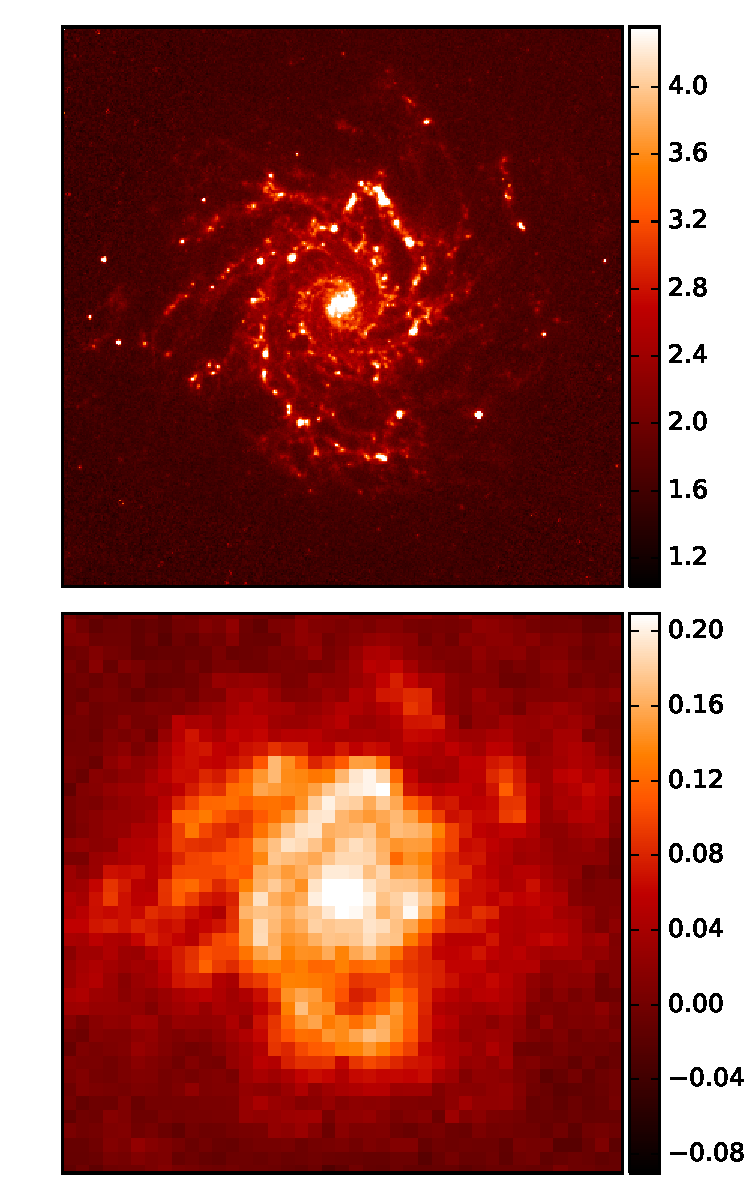
\includegraphics[width=0.9\linewidth]{figures/comparison.pdf}
    \caption[Spitzer and Herschel Observations]{Comparison of (top to bottom) Spitzer and Herschel observations of M74}
    \label{m74compare}
\end{figure}

By using the Spitzer observational data, it is then possible to create images for any telescope beam with a lower angular resolution than the original image. This can be done for instance, using the SPIRE beam, or a theoretical SPIRE beam for some imagined telescope with a larger primary mirror than Herschel. This allows the creation of both artificial observational data in the Herschel data processing pipeline, and theoretical higher resolution images for comparison.

\subsubsection{Overall Procedure}
The overall procedure for generating the simulation images is as follows:
\begin{enumerate}
    \item{Obtain the SPIRE $500\units{\mu m}$ observation data of M74}
    \item{Remove unused data products}
    \item{Obtain the Spitzer $24\units{\mu m}$ observation of M74}
    \item{Fourier convolve the Spitzer observation with the SPIRE $500\units{\mu m}$ beam}
    \item{Replace the timeline data in the SPIRE observation with the results from the Spitzer convolved image, manipulated with any noise background desired}
    \begin{enumerate}
        \item{Loop over each scan line}
        \item{Loop over each bolometer}
        \item{Loop over each data value and replace with corresponding convolved Spitzer data and noise data}
    \end{enumerate}
    \item{Build maps of simulated observation}
    \item{Build HiRes maps of the simulated data}
    \item{Create power spectra of both maps}
    \item{Create a truth image by convolving the original Spitzer data with a half-sized SPIRE beam}
\end{enumerate}

Both the nominal maps and HiRes maps can then be compared to the truth map in order to systematically study the performance of HiRes under any SNR conditions required. The method also extends as-is to the shorter wavelength observations, and observations of other objects.

\subsubsection{Creating a simulated Herschel Observation}

To generate the SPIRE observation, three primary components are needed:

\begin{enumerate}
    \item{An actual SPIRE observation to use as a data store}
    \item{An accurate SPIRE beam image}
    \item{The source Spitzer observation}
\end{enumerate}

The SPIRE observations are accessed using the HIPE software package \citep{HIPE}, and the particular observation of M74 can be found with an observation id of $1342189427$.

The beam for the long wave observations can be seen in Figure \ref{plwbeam}, and is known to very high accuracy. The Spitzer source image is shown in Figure \ref{m74compare}.

\begin{figure}[H]
    \centering
    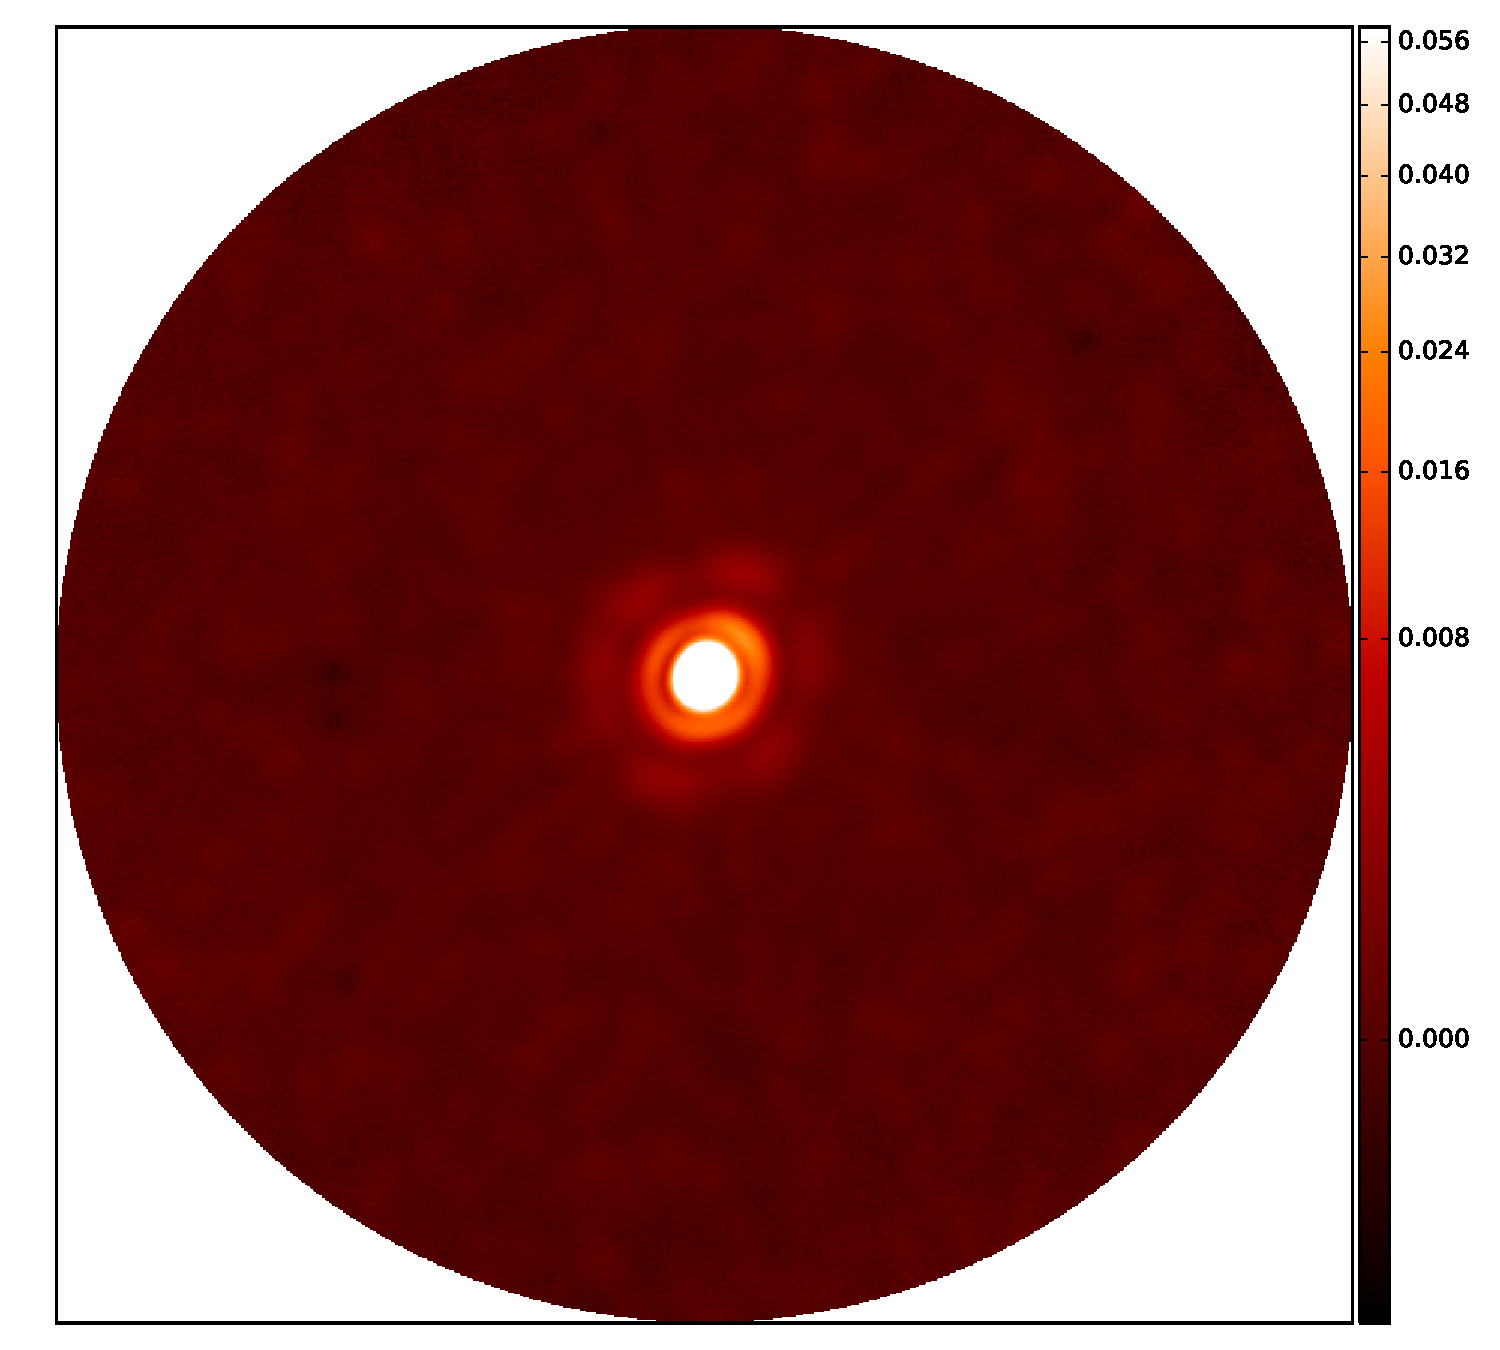
\includegraphics[width=0.8\linewidth]{figures/beam.pdf}
    \caption{SPIRE beam for $500\units{\mu m}$}
    \label{plwbeam}
\end{figure}

To create a variety of observations with varying levels of signal to noise, a dark sky observation was also chosen to provide sources of noise. While it would have been possible to artificially create random noise it was decided that using an actual source would give more realistic results. To do this we chose a wide angle observation of a 'dark' patch of sky (observation id of 1342186110) which can be sampled at various locations to generate different backgrounds for our created observation.

\subsubsection{Creating the Observations}

While I will be describing a high level overview of the process here, the actual code that generates the images can be found in the appendicies under '$spitzer.py$'.

To create any useful observational data, firstly the differences in units need to be considered. SPIRE observations, stored as a level 1 product in the HIPE software have timeline data stored in units of $\units{Jy/beam}$, and the Spitzer observations are stored in units of $\units{MJy/sr}$.

The first stage then is to convert the Spitzer data into units of $\units{Jy/pixel}$, this is done by the following operation:
\[ D = D \times 10^6 \times P \]
Where $D$ is the original image data, and $P$ is the factor necessary to convert from steradians to pixel size. In the case of these observations $P\simeq 3.8\e{-12}\units{pix/sr}$.

Next the Spitzer observation needs to be convolved with the SPIRE beam. First, the beam needs to be adjusted to have the same pixel resolution as the Spitzer image. This is done by creating a new WCS (world coordinate system) object and modifying it so that beam pixel grid resolution matches the source Spitzer image. HIPE has a tool called 'regrid' that performs this operation.

Secondly as the original beam image and Spitzer image contain NaN (invalid or no data) values, these need to be removed. In this pipeline the NaN values are removed simply by setting them to zero as they exist only at the outer regions of the beam image, and outside the area of interest in the Spitzer image. Once this has been completed, the beam and Spitzer image are transformed into Fourier space, multiplied together and then the resulting image transformed back into normal space giving a beam convolved image that now has data values in units of $\units{Jy/beam}$. NaN values can now be restored into the output image by taking the locations of NaN values in the source Spitzer image and applying them in the convolved image.

The background can the be removed from this convolved image by subtracting a median value from each pixel. Again due to there being NaN values in the image, the data needs to passed through a NaN filter before determining the background value.

Observational data in SPIRE data products is not simply stored as 2D image until mapping is performed. The data is stored in a series of time scans for each bolometer in the instrument. However as we have this timeline information in the SPIRE observation we can perform a simulation by altering this timeline data to data from a simulated scan of the Spitzer source image.

\begin{figure*}
    \centering
    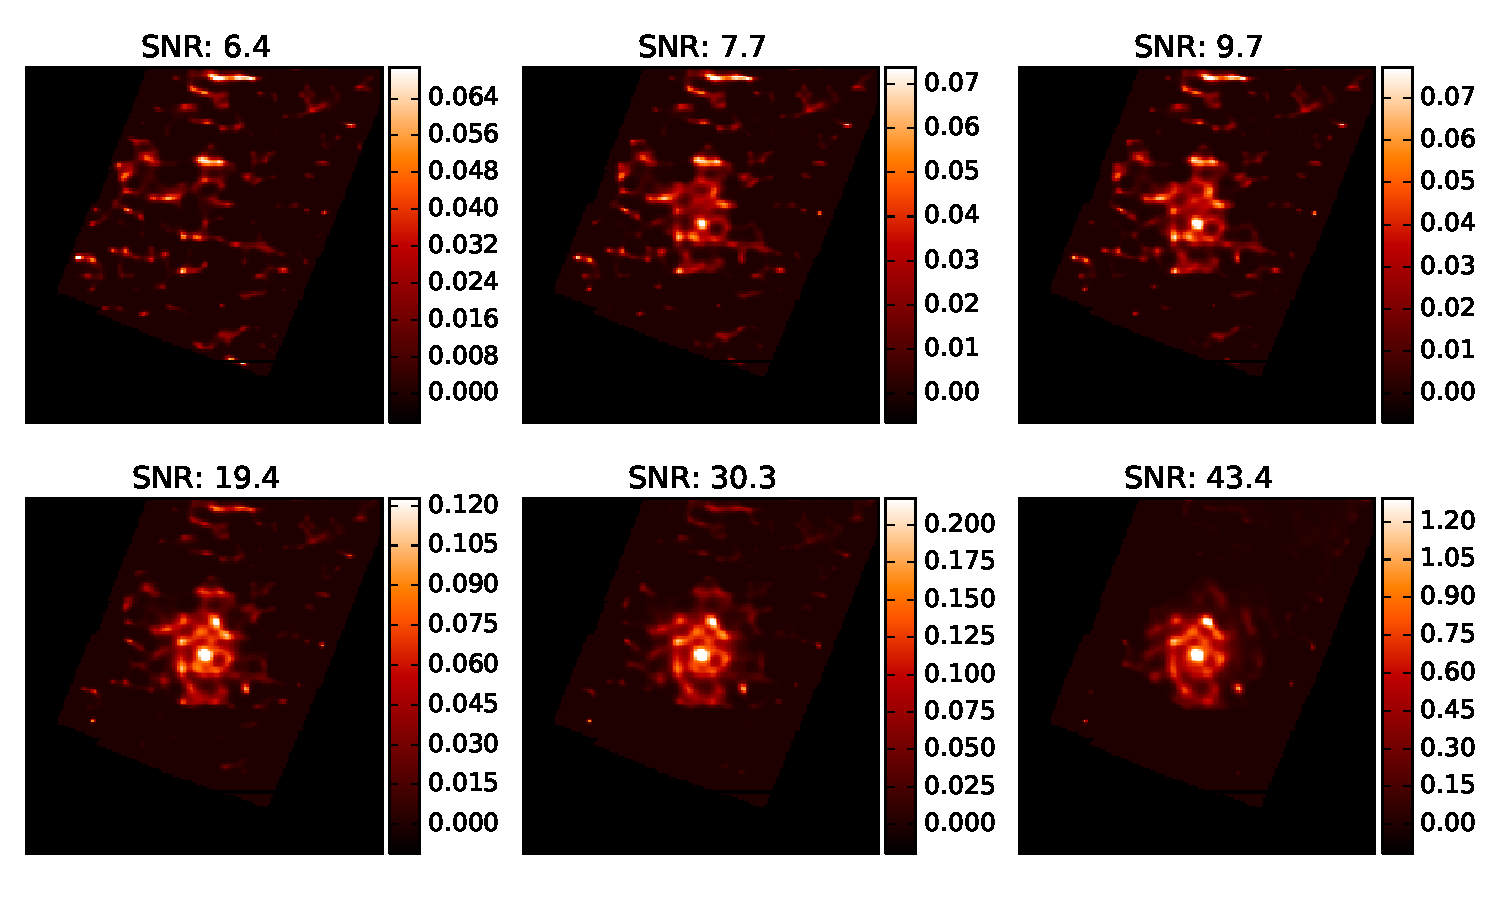
\includegraphics[width=0.9\linewidth]{figures/simulated-observations.pdf}
    \caption[Simulated observations]{Simulated observations at different signal to noise ratios, scale in Jy/beam}
    \label{simulatedobs}
\end{figure*}

To create observations with different levels of signal to noise, we also need to get the level 2 product of the chosen background source. This observation covers a much larger area than the M74 observation, so a set of locations is randomly chosen from which the background data can be obtained.

A scan line in a SPIRE observation contains data for each bolometer, and the data for each bolometer is stored as an array of signal values, with arrays for corresponding right ascension and declination values in the sky. The background value sky coordinates are obtained by taking a fixed point on the background image, with the difference from the sky coordinates of the start of the observation to the current position in the observation added to it. The Spitzer image value is obtained by simply getting the intensity at the location given by the sky coordinates in the SPIRE observation. The simulation is then performed by looping over each scan line, each bolometer and each signal value. The simulated observation intensity is then determined as
\[ D = B + I \times S \]
Where $D$ is the new observation data, $B$ is the background value, $I$ is the intensity in the Spitzer image and $S$ is the factor used to multiply the Spitzer value to give the desired signal to noise. This gives essentially an approximately fixed background noise level, to which any intensity of foreground to be added to create the images. Again NaN values need to be accounted for. Luckily these values only occur outside of the area of the observation that is being analyzed, so are again set to 0 to allow the mapping and HiRes enhancement to be performed.

Unfortunately it is not trivial to work out the SNR of the simulated image in advance, as the foreground already has it's own background noise that contributes. Instead the SNR must be determined after the image is created.

The above process is then repeated for each value of $S$ to generate a set of maps with different signal to noise ratios. Figure \ref{simulatedobs} shows how the image varies for different values of $S$.

Again, as previously mentioned this needs to be done for different background values so the effect of different features in the background can be eliminated. The whole process is repeated for different starting locations in the background images.

The end result is a set of images, both of the simulated observation and after performing HiRes, with varying signal to noise and using a variety of backgrounds. To generate this data for 9 different background locations, with 6 different signal to noise ratios each time and performing all the beam convolutions and HiRes processing takes around 6 hours on reasonably fast computer. Repeating for the higher resolution observations (medium and short wavelength) takes considerably longer, but the process is identical to that outlined above.

\subsubsection{Creating the Truth image for comparison}

To create a theoretical truth image for comparison, first the assumption is made that we can achieve around a two-fold increase in angular resolution through the use of HiRes. Again, as with the creation of the simulated Herschel observations we can use the same Spitzer image source.

Using the Herschel beam image, I create new beam that has the same properties and shape, but is half the size of the actual herschel beam, which corresponds to an identical optical system but with twice the angular resolution. To do this, I took the original beam FITS file, and altered the coordinate system so that the resulting beam has pixels with twice the angular size when mapped to sky coordinates. This is achieved by modifying the $cdelt$ property of the WCS coordinate system. This gives a beam image with the same pixel resolution, but twice the angular resolution so is in effect a beam for an equivalent telescope with twice the diameter aperture size.

Again, as with the generation of the observations, the source Spitzer image is then Fourier convolved with this new beam, giving an image that has twice the angular resolution of a Herchel observation, and should be the result of HiRes working on the simulated Herschel observations, again making the assumption that HiRes will at best give a resolution increase of a factor of two.

With this simulated truth image, there is now basis of comparison for determining how well HiRes has performed on any simulated observation, and can be compared to output images in a variety of ways.

\subsection{Storing the data for analysis}

To simplify analysis, the simulated observation, truth image and output of the HiRes routine are all saved out as FITS files. They are also coordinate aligned to show the same area of sky by matching the WCS coordinates between the three images. The data is also processd onto a new pixel grid so that each image has the same pixel resolution, chosen to match the HiRes output as this is the highest pixel resolution image created in the process. This has the advantage that pixel indices align between each image file, so comparisons can be made at a pixel level in the data, rather than having to worry about converting between sky coordinates and area coverage.

At this stage NaN values can also be restored by using the locations of NaNs in the original map before convolution, and replacing the locations in the simulated, HiRes and truth maps.

Power spectra are generated for each of the three maps, which are also saved as fits files, and the beam file returned by the HiRes routine is also saved in case this provides any useful information.

To provide a base noise image, one map is also generated containing just the noise background, without any of the Spitzer observation applied on top. The power spectra for this is also generated and saved.
